% replace all text with your own text.
% in this template few examples are mention
\chapter{Methodology}
\label{ch:method} % Label for method chapter

This chapter describes the objectives, scope, assumptions, limitations and the methods used to design and evaluate the air quality monitoring platform for Bogotá. Where possible, implementation details and parameter choices are drawn from the project workshops and the planned architecture described in earlier chapters.

%%%%%%%%%%%%%%%%%%%%%%%%%%%%%%%%%%%%%%%%%%%%%%%%%%%%%%%%%%%%%%%%%%%%%%%%%%%%%%%%%%%
\section{Objectives}
\label{sec:method_objectives}

The primary objective of this project is to design and implement a centralized, cloud-ready air quality monitoring platform that integrates real-time data from multiple sources and provides personalized, actionable health recommendations to citizens in Bogotá. The specific research and engineering objectives are:
\begin{enumerate}
    \item Design a scalable time-series database architecture based on PostgreSQL and TimescaleDB that supports monthly partitioning and efficient queries over multi-year datasets.
    \item Implement a robust data ingestion pipeline that collects heterogeneous data from AQICN, Google Air Quality API, and IQAir at 10-minute intervals and stores raw payloads in MinIO for audit and replay.
    \item Define a normalization schema and ETL process that harmonizes units, field names and AQI scales into a unified relational schema.
    \item Implement query acceleration using concurrently refreshed materialized views and appropriate indexing strategies to meet target latency goals (p95 < 2s under 1000 concurrent users).
    \item Provide an API layer (REST + GraphQL) that serves dashboards, researcher exports (CSV), and programmatic integrations.
    \item Develop a rule-based recommendation engine that maps AQI categories and user metadata into personalized health advice and product suggestions.
    \item Validate the system against planned performance tests and document lessons learned for future scaling and predictive extensions.
\end{enumerate}

%%%%%%%%%%%%%%%%%%%%%%%%%%%%%%%%%%%%%%%%%%%%%%%%%%%%%%%%%%%%%%%%%%%%%%%%%%%%%%%%%%%
\section{Scope}
\label{sec:method_scope}

This project focuses on a single-city deployment (Bogotá) with an initial historical dataset covering 2022--2024. The scope includes:
\begin{itemize}
    \item Collection of air quality observations from external APIs (AQICN, Google Air Quality, IQAir) and local government sources where available.
    \item Storage of raw JSON payloads in MinIO and normalized records in a PostgreSQL/TimescaleDB hypertable partitioned by month and city.
    \item Implementation of a recommendation engine based on AQI thresholds and user-provided risk profiles.
    \item Implementation of an API layer and basic dashboard endpoints for citizens and researchers.
    \item Performance validation using planned JMeter load tests and Prometheus/Grafana monitoring.
\end{itemize}

Exclusions (out of scope for the current phase):
\begin{itemize}
    \item Real-time high-frequency (sub-minute) ingestion; the current architecture targets 10-minute ingestion intervals.
    \item Full-scale distributed stream-processing fabrics (Kafka/Flink) are not implemented in the baseline but are described as future extensions.
    \item Clinical validation of health recommendations with medical professionals (recommendations are based on public guidelines and should not replace medical advice).
    \item Multi-city production deployment—this is left as future work after Bogotá evaluation.
\end{itemize}

%%%%%%%%%%%%%%%%%%%%%%%%%%%%%%%%%%%%%%%%%%%%%%%%%%%%%%%%%%%%%%%%%%%%%%%%%%%%%%%%%%%
\section{Assumptions}
\label{sec:method_assumptions}

The following assumptions guided the design and evaluation:
\begin{itemize}
    \item External APIs (AQICN, Google, IQAir) provide consistent identifiers for stations and timestamps in UTC or include timezone information that can be normalized.
    \item Ingestion at 10-minute intervals is sufficient for citizen-oriented recommendations and dashboard responsiveness for the Bogotá use case.
    \item Historical CSV archives (2022--2024) are representative for initial benchmarking and performance validation.
    \item Users can supply minimal profile information (location, activity preferences, basic health risk flags) to enable personalization without requiring sensitive medical records.
    \item The deployment environment will provide at least the planned hardware profile for performance testing (e.g., 4 vCPU, 16 GB RAM for the primary database node).
\end{itemize}

%%%%%%%%%%%%%%%%%%%%%%%%%%%%%%%%%%%%%%%%%%%%%%%%%%%%%%%%%%%%%%%%%%%%%%%%%%%%%%%%%%%
\section{Limitations}
\label{sec:method_limitations}

This project has several limitations that affect interpretation and generalization of the results:
\begin{itemize}
    \item Data availability and API quotas may limit continuous ingestion from third-party providers; historical archives reduce but do not eliminate this constraint.
    \item The recommendation engine is rule-based and deterministic; it does not incorporate personalized predictive models or machine-learning-driven forecasting in the baseline.
    \item Sensor calibration and data quality from heterogeneous sources remain a challenge; low-cost sensors may introduce bias and require calibration procedures outside the initial scope.
    \item The performance targets assume a modest single-node deployment; results may differ on constrained hardware or cloud instances with different I/O characteristics.
    \item Ethical and clinical validation of health advice is outside the project's scope; recommendations should be treated as informational rather than clinical directives.
\end{itemize}

%%%%%%%%%%%%%%%%%%%%%%%%%%%%%%%%%%%%%%%%%%%%%%%%%%%%%%%%%%%%%%%%%%%%%%%%%%%%%%%%%%%
\section{Methodology}
\label{sec:method_method}

This section details the methods, data flows, and experimental procedures used to design, implement, and validate the system. The methodology is organized by functional component: data ingestion, normalization and storage, query acceleration, API layer, recommendation engine, and performance validation.

\subsection{Data Ingestion}
\label{subsec:method_ingest}

Data is collected by a Python-based ingestion service configured to poll selected external APIs every 10 minutes. Each poll performs the following steps:
\begin{enumerate}
    \item Retrieve JSON payloads for Bogotá and related stations from AQICN, Google Air Quality API, and IQAir endpoints.
    \item Persist the raw JSON to MinIO under a versioned key with schema: \texttt{raw-airquality/YYYY/MM/DD/HHMM\_source\_station.json} for auditability and reprocessing.
    \item Emit a lightweight validation check (schema presence, timestamp parseable, sensor id) and place invalid payloads into a quarantine bucket for manual inspection.
    \item Forward valid payloads to the normalizer via an in-process call (or message queue in future iterations).
\end{enumerate}

\subsection{Normalization and Storage}
\label{subsec:method_normalization}

The normalizer maps each provider-specific payload to a unified relational schema. Key steps:
\begin{itemize}
    \item Field mapping: provider fields (for example, \texttt{pm25}, \texttt{PM2\_5} or \texttt{pm\_2\_5}) are normalized to the canonical column name \texttt{pm25}.
    \item Unit harmonization: concentrations are converted to standard units (\(\mu\)g/m\(^{3}\)) where necessary.
    \item AQI conversion: when providers publish different AQI scales, the normalizer converts pollutant concentrations into the chosen standard AQI scale (EPA or WHO mappings) to keep recommendations consistent.
    \item Persistence: insert normalized records into the \texttt{airquality\_reading} hypertable partitioned by month and city (TimescaleDB). Each insert is executed in a short transaction and uses identifiers such as \texttt{station\_id} and \texttt{pollutant\_id} with a uniqueness constraint on (\texttt{station\_id}, \texttt{pollutant\_id}, \texttt{datetime}) to avoid duplicates.
\end{itemize}

\subsection{Query Acceleration and Indexing}
\label{subsec:method_query}

To support sub-2-second p95 latency targets the system uses multiple optimization techniques:
\begin{itemize}
    \item Concurrently refreshed materialized views for pre-computed aggregation windows (15-minute, hourly, daily) and for common dashboard queries.
    \item Composite B-tree indexes on (\texttt{timestamp}, \texttt{station\_id}, \texttt{pollutant\_id}) and partial indexes that cover recent data (for example, the last 30 days).
    \item BRIN indexes for very large historical partitions; BRIN reduces index size and maintenance overhead for old chunks.
    \item TimescaleDB continuous aggregates for frequently requested rollups to reduce on-demand computation costs.
\end{itemize}

\subsection{API Layer and Services}
\label{subsec:method_api}

The API layer exposes both REST and GraphQL endpoints. Key design choices:
\begin{itemize}
    \item Authentication: lightweight token-based authentication for researchers and admin users; public endpoints for citizen dashboards limit per-IP rate to protect upstream APIs and database load.
    \item Endpoints: summary endpoints for current AQI, rolling-window endpoints for time series (GraphQL supports nested queries), and CSV export endpoints for researchers.
    \item Observability: Prometheus metrics exposed for ingest latency, API response times, materialized view refresh duration, and DB query statistics; Grafana dashboards visualize these metrics.
\end{itemize}

\subsection{Recommendation Engine}
\label{subsec:method_reco}

The recommendation engine is rule-based and deterministic. Implementation highlights:
\begin{itemize}
    \item Input: latest AQI per location, user profile (age bracket, respiratory risk flag, activity preference), and optional device location.
    \item Rule set: AQI category lookup table (EPA bands) maps to health advice templates. Rules include thresholds for protective product suggestions (for example, recommend N95 when AQI $\geq$ 151 for outdoor exercise).
    \item Delivery: notifications via email or push; caching layer prevents repeated alerts for unchanged AQI categories within a 3-hour TTL unless user location changes by $>2\,$km.
    \item Explainability: each recommendation includes the rule identifier and the AQI/pollutant evidence used to derive it to enable user transparency.
\end{itemize}

\subsection{Performance Validation and Experiments}
\label{subsec:method_experiments}

Planned experiments to validate system properties:
\begin{itemize}
    \item \textbf{Dataset ingestion}: ingest three years (2022--2024) of Bogotá historical data into the hypertable and measure storage growth and ingest throughput.
    \item \textbf{Load testing}: use Apache JMeter to simulate up to 1000 concurrent users issuing dashboard and CSV-export requests. Measure p95 latency, throughput, CPU and I/O utilization.
    \item \textbf{Materialized view refresh tests}: measure refresh duration of key views under varying chunk sizes and concurrency; tune chunk time intervals and refresh schedule based on results.
    \item \textbf{Fault-injection}: emulate API downtime and delayed ingestion to validate replay from MinIO and quarantine/reprocessing procedures.
\end{itemize}

\section{Summary}

This methodology chapter documents the concrete steps and design choices used to build an end-to-end air quality monitoring platform for Bogotá. The following chapter details the implementation and experimental results obtained while evaluating the proposed system. Table~\ref{tab:gen_template} describes that, in general, a typical report structure has three main parts: (1) front matter, (2) main text, and (3) end matter. %[\textbf{also notice that the preceding sentence is an example of a numbered list in a text body}]. 
The structure of the front matter and end matter will remain the same for all the undergraduate final year project report. However, the main text varies as per the project's needs.
\begin{table}[!ht]
    \centering
    \caption{Undergraduate report template structure}
    \label{tab:gen_template}
    \begin{tabular}{llll}     
        \toprule
        \multirow{7}{3cm}{Frontmatter} 
        & & Title Page & \\                  
        & & Abstract &    \\          
        & & Acknowledgements & \\                            
        & & Table of Contents &    \\                                
        & & List of Figures   &    \\                        
        & & List of Tables    &    \\                
        & & List of Abbreviations  &    \\                     
        & &   &    \\                        
        \multirow{7}{3cm}{Main text}
        & Chapter 1 & Introduction   &    \\                         
        & Chapter 2 & Literature Review   &    \\
        & Chapter 3 & Methodology   &    \\
        & Chapter 4 & Results    &    \\
        & Chapter 5 & Discussion and Analysis  &    \\
        & Chapter 6 & Conclusions and Future Work  &    \\        
        & Chapter 7 & Refection  &    \\          
        & &   &    \\                       
        \multirow{2}{3cm}{End matter}
        & & References  &    \\   
        & & Appendices (Optional)  &    \\ 
        & & Index (Optional)  &    \\ 
        \bottomrule
    \end{tabular}
\end{table}

\subsection{Example of a software/Web development main text structure}
\label{subsec:se_chpters}
Notice that the ``methodology'' Chapter of Software/Web development in Table~\ref{tab:soft_eng_temp} takes a standard software engineering paradigm (approach). Alternatively, these suggested sections can be the chapters of their own. Also, notice that ``Chapter 5'' in Table~\ref{tab:soft_eng_temp} is ``Testing and Validation'' which is different from the general report template mentioned in Table~\ref{tab:gen_template}. Check with your supervisor if in doubt.
\begin{table}[!ht]
    \centering
    \caption{Example of a software engineering-type report structure}
    \label{tab:soft_eng_temp}
    \begin{tabular}{lll}     
        \toprule                   
        Chapter 1 & Introduction   &    \\        
        Chapter 2 & Literature Review  &    \\                   
        Chapter 3 & Methodology   &    \\
        &               & Requirements specifications   \\
        &               & Analysis   \\
        &               & Design   \\
        &               & Implementations   \\
        Chapter 4 & Testing and Validation  &    \\
        Chapter 5 & Results and Discussion      &    \\
        Chapter 6 & Conclusions and Future Work  &    \\        
        Chapter 7 & Reflection  &    \\                          
        \bottomrule
    \end{tabular}
\end{table}

\subsection{Example of an algorithm analysis main text structure}
Some project might involve the implementation of a state-of-the-art algorithm and its performance analysis and comparison with other algorithms. In that case, the suggestion in Table~\ref{tab:algo_temp} may suit you the best. 
\begin{table}[!ht]
    \centering
    \caption{Example of an algorithm analysis type report structure}
    \label{tab:algo_temp}
    \begin{tabular}{lll}     
        \toprule                   
        Chapter 1 & Introduction  &    \\        
        Chapter 2 & Literature Review  &    \\                
        Chapter 3 & Methodology   &    \\
        &               & Algorithms descriptions  \\
        &               & Implementations   \\
        &               & Experiments design   \\
        Chapter 4 & Results       &  \\
        Chapter 5 & Discussion and Analysis  &    \\
        Chapter 6 & Conclusion and Future Work  &    \\        
        Chapter 7 & Reflection  &    \\          
        \bottomrule
    \end{tabular}
\end{table}

\subsection{Example of an application type main text structure}
If you are applying some algorithms/tools/technologies on some problems/datasets/etc., you may use the methodology section prescribed in Table~\ref{tab:app_temp}.  
\begin{table}[!ht]
    \centering
    \caption{Example of an application type report structure}
    \label{tab:app_temp}
    \begin{tabular}{lll}     
        \toprule                   
        Chapter 1 & Introduction  &    \\        
        Chapter 2 & Literature Review  &    \\                
        Chapter 3 & Methodology   &    \\
        &               & Problems (tasks) descriptions  \\
        &               & Algorithms/tools/technologies/etc. descriptions  \\        
        &               & Implementations   \\
        &               & Experiments design and setup   \\
        Chapter 4 & Results       &  \\
        Chapter 5 & Discussion and Analysis  &    \\
        Chapter 6 & Conclusion and Future Work  &    \\        
        Chapter 7 & Reflection  &    \\          
        \bottomrule
    \end{tabular}
\end{table}

\subsection{Example of a science lab-type main text structure}
If you are doing a science lab experiment type of project, you may use the  methodology section suggested in Table~\ref{tab:lab_temp}. In this kind of project, you may refer to the ``Methodology'' section as ``Materials and Methods.''
\begin{table}[!ht]
    \centering
    \caption{Example of a science lab experiment-type report structure}
    \label{tab:lab_temp}
    \begin{tabular}{lll}     
        \toprule                   
        Chapter 1 & Introduction  &    \\        
        Chapter 2 & Literature Review  &    \\                
        Chapter 3 & Materials and Methods   &    \\
        &               & Problems (tasks) description  \\
        &               & Materials \\        
        &               & Procedures  \\                
        &               & Implementations   \\
        &               & Experiment set-up   \\
        Chapter 4 & Results       &  \\
        Chapter 5 & Discussion and Analysis  &    \\
        Chapter 6 & Conclusion and Future Work  &    \\        
        Chapter 7 & Reflection  &    \\          
        \bottomrule
    \end{tabular}
\end{table}

\subsection{Ethical considerations}
This section addresses ethical aspects of your project. This may include:
    informed consent, describing how participants will be informed about the study's purpose, procedures, risks, and benefits. You should detail the process used for obtaining consent and ensuring participants understand their rights.


\begin{itemize}
    \item \textbf{Informed Consent}: If data was collected from participant, detail the process for obtaining consent and ensuring participants understand their rights.
    
    \item \textbf{Confidentiality and Privacy}: Explain measures taken to protect participants' data and maintain confidentiality. Discuss how data is stored, who will have access, and how anonymity will be preserved.
    
    \item \textbf{Risk Assessment}: Identify potential risks to participants and outline strategies to minimize them. 
    
    \item \textbf{Vulnerable Populations}: If applicable, address how you will protect vulnerable groups (e.g., children, elderly, or marginalized communities) involved in your project. 
    
    \item \textbf{Research Integrity}: Highlight your commitment to honesty and transparency in research. Discuss how you will avoid plagiarism, fabrication, and falsification of data.
    
    \item \textbf{Compliance with Regulations}: Mention relevant ethical guidelines and regulations that your project will adhere to.
    
    \item \textbf{Impact on Society}: Reflect on the broader implications of your project. Discuss how the outcomes may affect communities, stakeholders, or the environment, and how you plan to address any potential negative consequences.
    
    \item \textbf{Feedback Mechanisms}: Describe how you incorporate feedback from participants and stakeholders to improve the ethical conduct of the project throughout its duration.

\end{itemize}


\section{Example of an Equation in \LaTeX}
Eq.~\ref{eq:eq_example} [note that this is an example of an equation's in-text citation] is an example of an equation in \LaTeX. In Eq.~\eqref{eq:eq_example}, $ s $ is the mean of elements $ x_i \in \mathbf{x} $: 

\begin{equation}
\label{eq:eq_example} % label used to refer the eq in text
s = \frac{1}{N} \sum_{i = 1}^{N} x_i. 
\end{equation}

Have you noticed that all the variables of the equation are defined using the \textbf{in-text} maths command \$.\$, and Eq.~\eqref{eq:eq_example} is treated as a part of the sentence with proper punctuation? Always treat an equation or expression as a part of the sentence. 



\section{Example of a Figure in \LaTeX}
Figure~\ref{fig:chart_a} is an example of a figure in \LaTeX. For more details, check the link:

\href{https://en.wikibooks.org/wiki/LaTeX/Floats,_Figures_and_Captions}{wikibooks.org/wiki/LaTeX/Floats,\_Figures\_and\_Captions}.

\noindent
Keep your artwork (graphics, figures, illustrations) clean and readable. At least 300dpi is a good resolution of a PNG format artwork. However, an SVG format artwork saved as a PDF will produce the best quality graphics. There are numerous tools out there that can produce vector graphics and let you save that as an SVG file and/or as a PDF file. One example of such a tool is the ``Flow algorithm software''. Here is the link for that: \href{http://www.flowgorithm.org/download/}{flowgorithm.org}.
\begin{figure}[!ht]
    \centering
    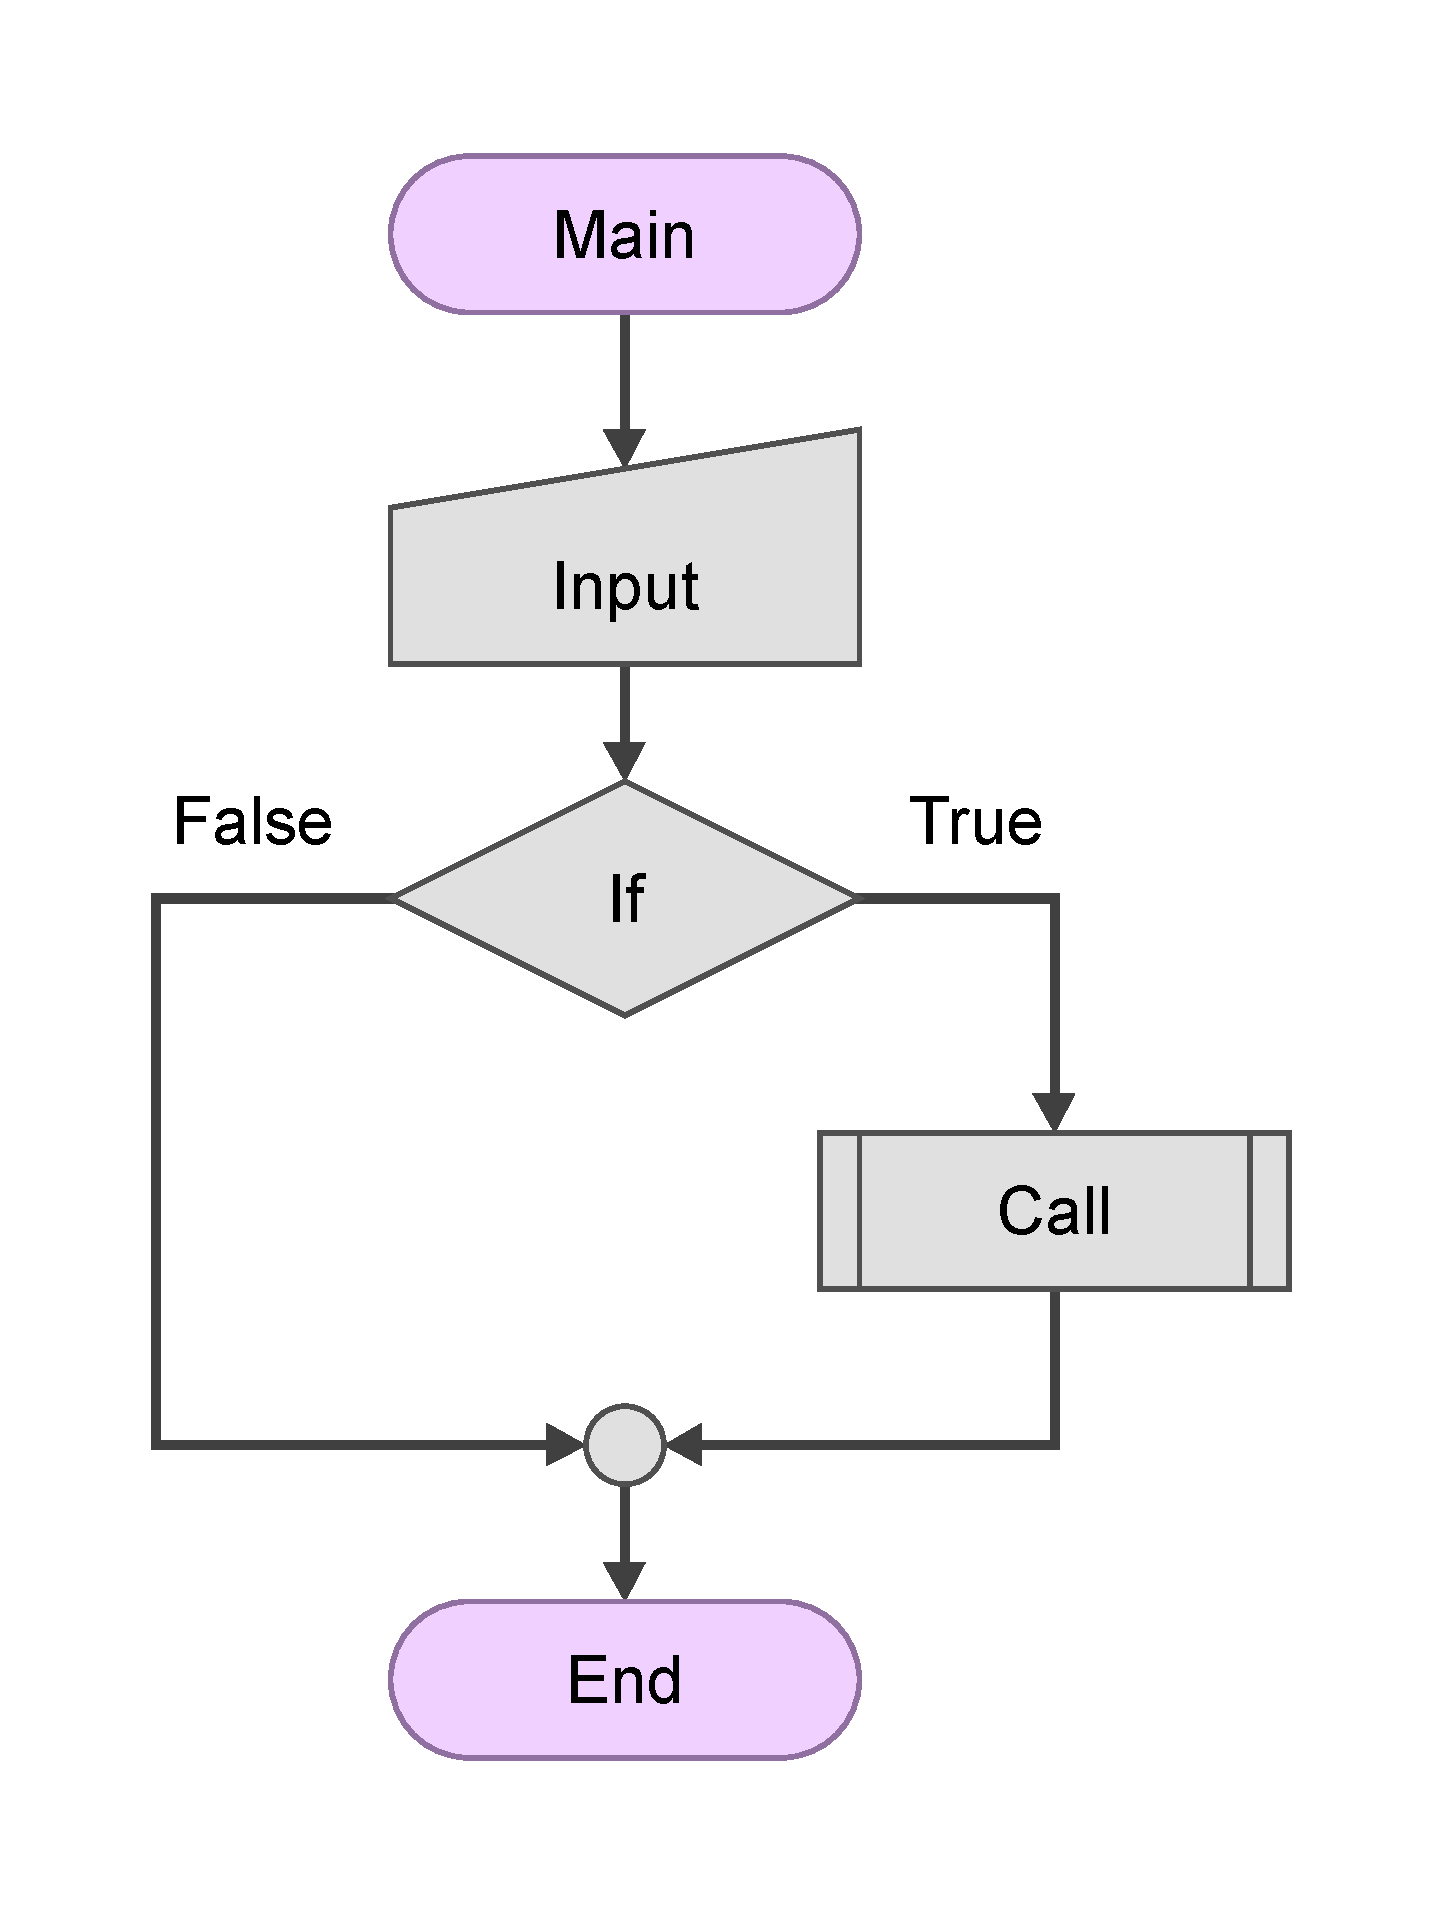
\includegraphics[scale=0.3]{figures/chart.pdf}
    \caption{Example figure in \LaTeX.}
    \label{fig:chart_a}
\end{figure}

\clearpage %  use command \clearpage when you want section or text to appear in the next page.

\section{Example of an algorithm in \LaTeX}
Algorithm~\ref{algo:algo_example} is a good example of an algorithm in \LaTeX.  
\begin{algorithm}
    \caption{Example caption: sum of all even numbers}
    \label{algo:algo_example}
    \begin{algorithmic}[1]
        \Require{$ \mathbf{x}  = x_1, x_2, \ldots, x_N$}
        \Ensure{$EvenSum$ (Sum of even numbers in $ \mathbf{x} $)}
        \Statex
        \Function{EvenSummation}{$\mathbf{x}$}
        \State {$EvenSum$ $\gets$ {$0$}}
        \State {$N$ $\gets$ {$length(\mathbf{x})$}}
        \For{$i \gets 1$ to $N$}                    
        \If{$ x_i\mod 2 == 0$}  \Comment Check whether a number is even.
        \State {$EvenSum$ $\gets$ {$EvenSum + x_i$}}
        \EndIf
        \EndFor
        \State \Return {$EvenSum$}
        \EndFunction
    \end{algorithmic}
\end{algorithm}
 
\section{Example of code snippet  in \LaTeX}

Code Listing~\ref{list:python_code_ex} is a good example of including a code snippet in a report. While using code snippets, take care of the following:
\begin{itemize}
    \item do not paste your entire code (implementation) or everything you have coded. Add code snippets only. 
    \item The algorithm shown in Algorithm~\ref{algo:algo_example} is usually preferred over code snippets in a technical/scientific report. 
    \item Make sure the entire code snippet or algorithm stays on a single page and does not overflow to another page(s).  
\end{itemize}

Here are three examples of code snippets for three different languages (Python, Java, and CPP) illustrated in Listings~\ref{list:python_code_ex}, \ref{list:java_code_ex}, and \ref{list:cpp_code_ex} respectively.  

\begin{lstlisting}[language=Python, caption={Code snippet in \LaTeX ~and  this is a Python code example}, label=list:python_code_ex]
import numpy as np

x  = [0, 1, 2, 3, 4, 5] # assign values to an array
evenSum = evenSummation(x) # call a function

def evenSummation(x):
    evenSum = 0
    n = len(x)
    for i in range(n):
        if np.mod(x[i],2) == 0: # check if a number is even?
            evenSum = evenSum + x[i]
    return evenSum
\end{lstlisting}

Here we used  the ``\textbackslash clearpage'' command and forced-out the second listing example onto the next page. 
\clearpage  %
\begin{lstlisting}[language=Java, caption={Code snippet in \LaTeX ~and  this is a Java code example}, label=list:java_code_ex]
public class EvenSum{ 
    public static int evenSummation(int[] x){
        int evenSum = 0;
        int n = x.length;
        for(int i = 0; i < n; i++){
            if(x[i]%2 == 0){ // check if a number is even?
                evenSum = evenSum + x[i];
            }
        }
        return evenSum;     
    }
    public static void main(String[] args){ 
        int[] x  = {0, 1, 2, 3, 4, 5}; // assign values to an array
        int evenSum = evenSummation(x);
        System.out.println(evenSum);
    } 
} 
\end{lstlisting}


\begin{lstlisting}[language=C, caption={Code snippet in \LaTeX ~and  this is a C/C++ code example}, label=list:cpp_code_ex]
int evenSummation(int x[]){
    int evenSum = 0;
    int n = sizeof(x);
    for(int i = 0; i < n; i++){
        if(x[i]%2 == 0){ // check if a number is even?
            evenSum = evenSum + x[i];
    	}
    }
    return evenSum;     
}

int main(){
    int x[]  = {0, 1, 2, 3, 4, 5}; // assign values to an array
    int evenSum = evenSummation(x);
    cout<<evenSum;
    return 0;
}
\end{lstlisting}



\section{Example of in-text citation style}
\subsection{Example of the equations and illustrations placement and reference in the text}
Make sure whenever you refer to the equations, tables, figures, algorithms,  and listings for the first time, they also appear (placed) somewhere on the same page or in the following page(s). Always make sure to refer to the equations, tables and figures used in the report. Do not leave them without an \textbf{in-text citation}. You can refer to equations, tables and figures more them once.

\subsection{Example of the equations and illustrations style}
Write \textbf{Eq.} with an uppercase ``Eq`` for an equation before using an equation number with (\textbackslash eqref\{.\}). Use ``Table'' to refer to a table, ``Figure'' to refer to a figure, ``Algorithm'' to refer to an algorithm and ``Listing'' to refer to listings (code snippets). Note that, we do not use the articles ``a,'' ``an,'' and ``the'' before the words Eq., Figure, Table, and Listing, but you may use an article for referring the words figure, table, etc. in general.

For example, the sentence ``A report structure is shown in \textbf{the} Table~\ref{tab:gen_template}'' should be written as ``A report structure is shown \textbf{in} Table~\ref{tab:gen_template}.'' 

\subsection{Tools for In-text Referencing}\label{subsec:reftools}
You will have noticed that there are linked references within the text to specific items in this document (e.g., equations, figures, tables, chapters, sections, etc.).  This is enabled by a combination of \verb|\label{}| and \verb|\ref{}| commands.  The former is typically ``attached'' to an object/section to be labeled, for instance: \lstinline!\section{My Section}\label{sec:my}!.  This label, \verb|sec:my|, can then be used to create an in-text reference (with link) to the referenced object: \verb|\ref{sec:my}|.

The in-text references to the preceding equation were written as: \lstinline!Eq.~\eqref{eq:eq_example}!.  Here, the author needed to explicitly write the \verb|Eq.| text, include a tilde, \verb|~|, to ensure that the text is not separated from the number at a line break, and used \verb|eqref| to automate placement of parentheses around the number.  Alternatively, we could use the cleverref system to reference this item with \verb|\Cref{eq:eq_example}|, yielding: \Cref{eq:eq_example}.  This makes the textual part (Equation) automatic along with spacing and other formatting.  The capital \verb|C| in that command specifies capitalisation of the word, whereas lowercase for a figure item would, \verb|\cref{fig:chart_a}| would yield a lowercase abbreviated form: \cref{fig:chart_a}.

\section{Summary}
Write a summary of this chapter.

~\\[5em]
\noindent
{\huge\textbf{Note:}} In the case of \textbf{software engineering} project a Chapter ``\textbf{Testing and Validation}'' should precede the ``Results'' chapter. See Section~\ref{subsec:se_chpters} for report organization of such project. 

